\section{Objectif}

\subsection{Archétype}
    L'objectif du projet est de réaliser un jeu s'inspirant du jeu de stratégie Risk, avec des règles simplifiées.
    
\subsection{Règles du jeu}
    Au début du jeu, le joueur reçoit des territoires puis gère ses armées en les plaçant sur les pays qu'ils possèdent. A tour de rôle, les deux adversaires s'attaquent afin de gagner des territoires. Le vainqueur est celui qui conquiert tous les territoires ennemis (nous pourrons modifier cet aspect du jeu pour que les parties durent moins longtemps). Pour cela, il doit lancer des dés qui décideront de l'issue du combat sur un territoire donné. Le joueur peut perdre des armées à chaque phase de jeu et reçoit quelques unités de combat à diverses occasions. 

\subsection{Ressources}
    Plusieurs ressources sont nécessaires pour afficher l'état du jeu au cours de la partie. 
    Le joueur joue sur un plateau représentant le monde. Chaque continent est représenté par une couleur.  (figure \ref{fig:textures_plateau} et figure \ref{fig:textures_plateau2}).  Les armées sont représentées par des pions (figure \ref{fig:textures_pions}). Le nombre d'armées par territoire sera indiqué par un nombre. Enfin, lorsqu'il conquiert un territoire, le joueur reçoit une carte qui pourra lui donner des avantages. (figure \ref{fig:textures_cartes}). Les éléments ressources seront améliorés au fur et à mesure de la conception. 
    
    \begin{figure}[!htbp]
        \centering
        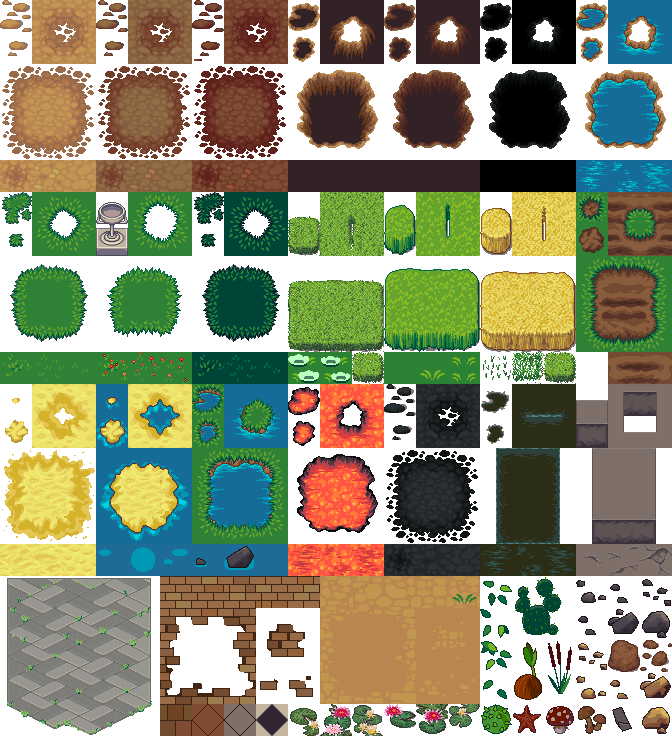
\includegraphics[width=6cm]{Images/terrain.png}
        \caption{Textures pour la plateau}
        \label{fig:textures_plateau}
    \end{figure}
    \newpage
    
    \begin{figure}[!htbp]
        \centering
        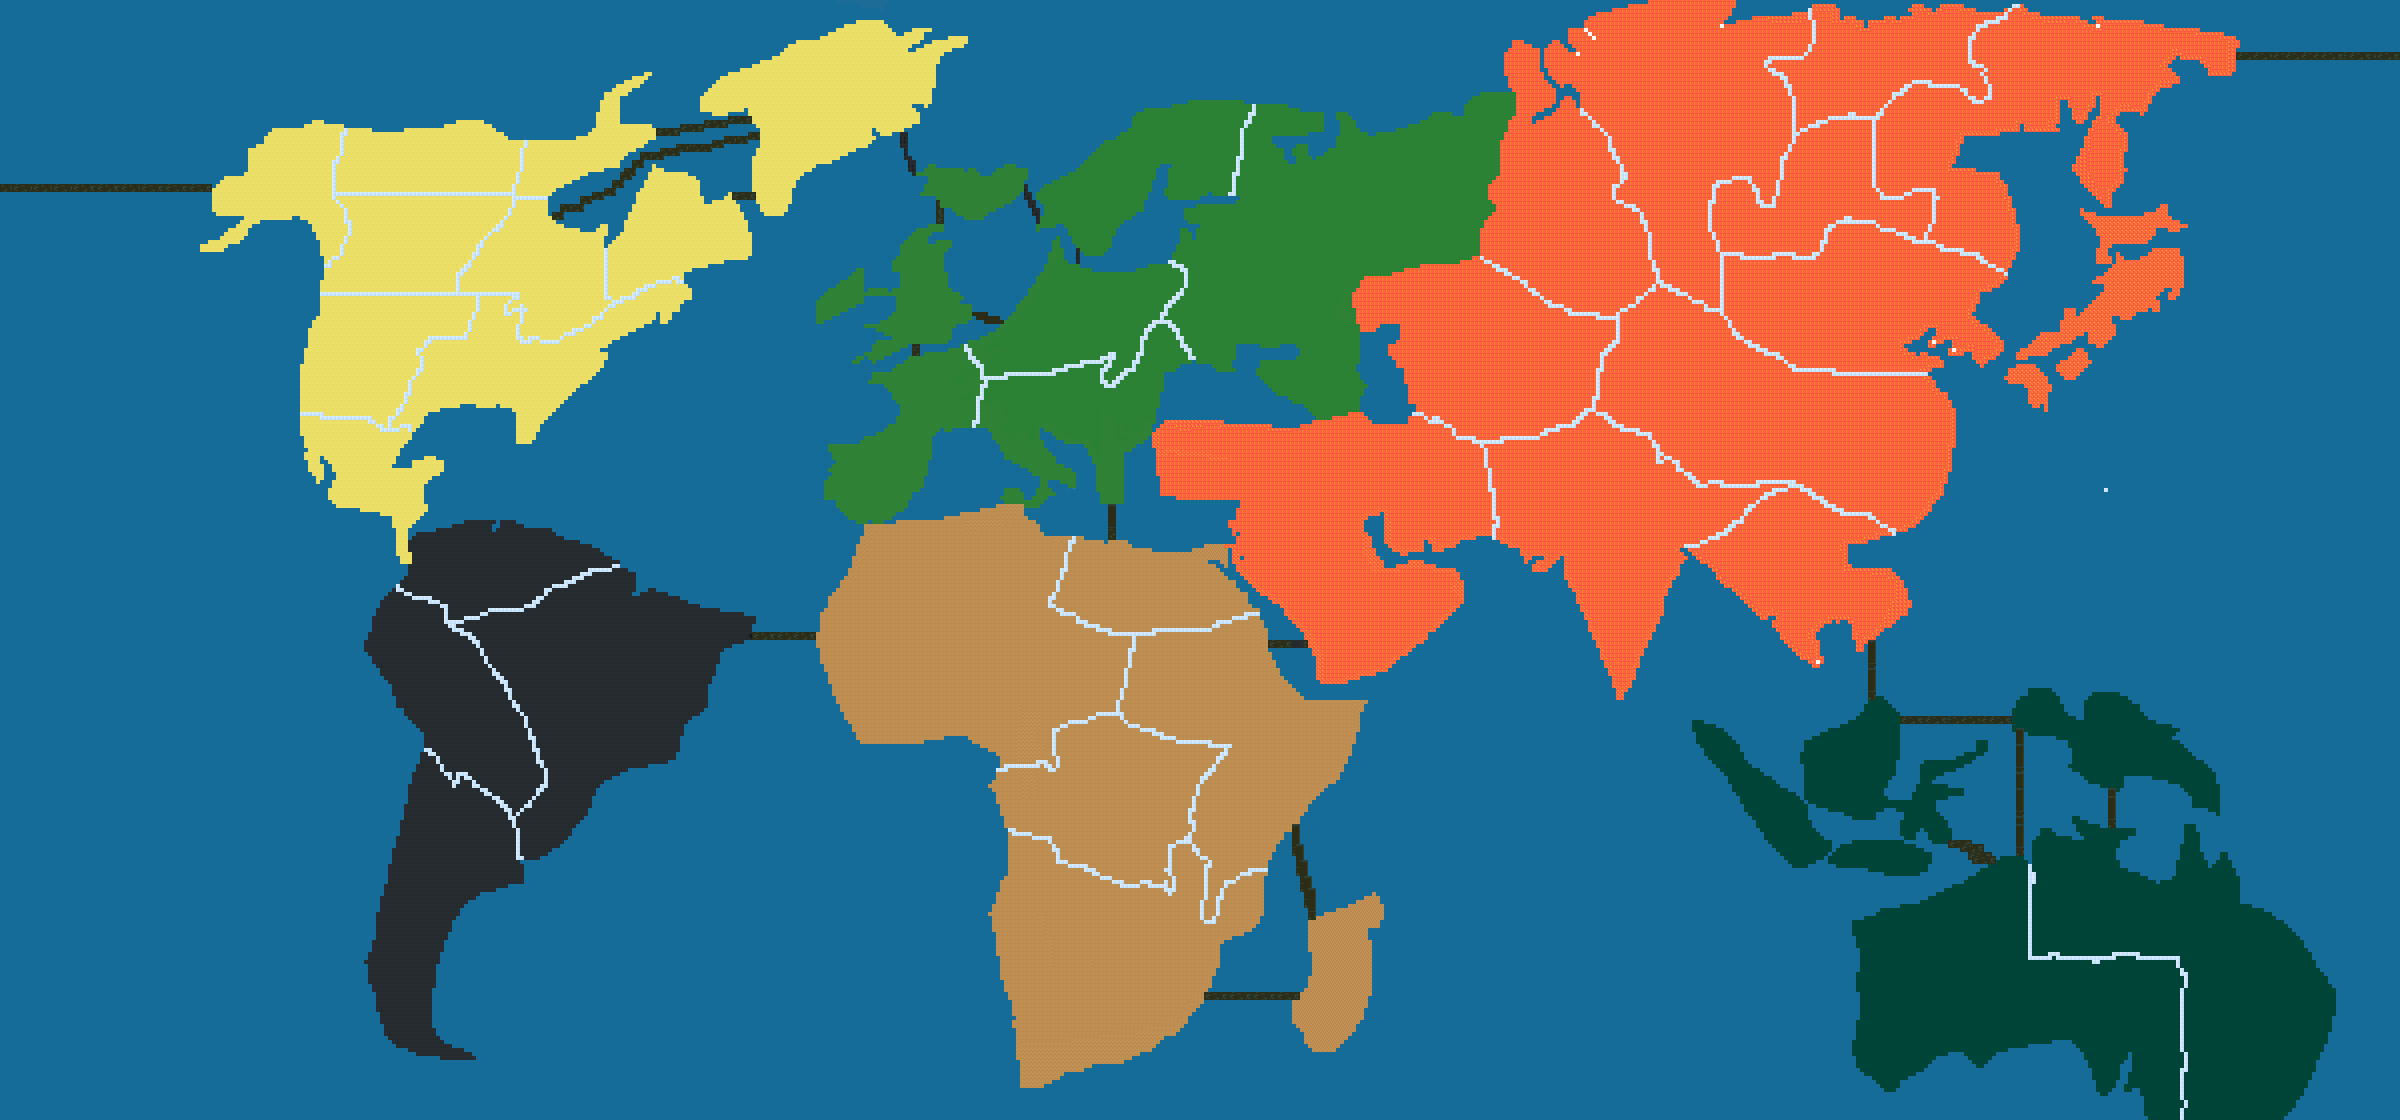
\includegraphics[width=13cm]{Images/map_jeu.png}
        \caption{Textures pour la plateau}
        \label{fig:textures_plateau2}
    \end{figure}
    
    \begin{figure}[!htbp]
        \centering
        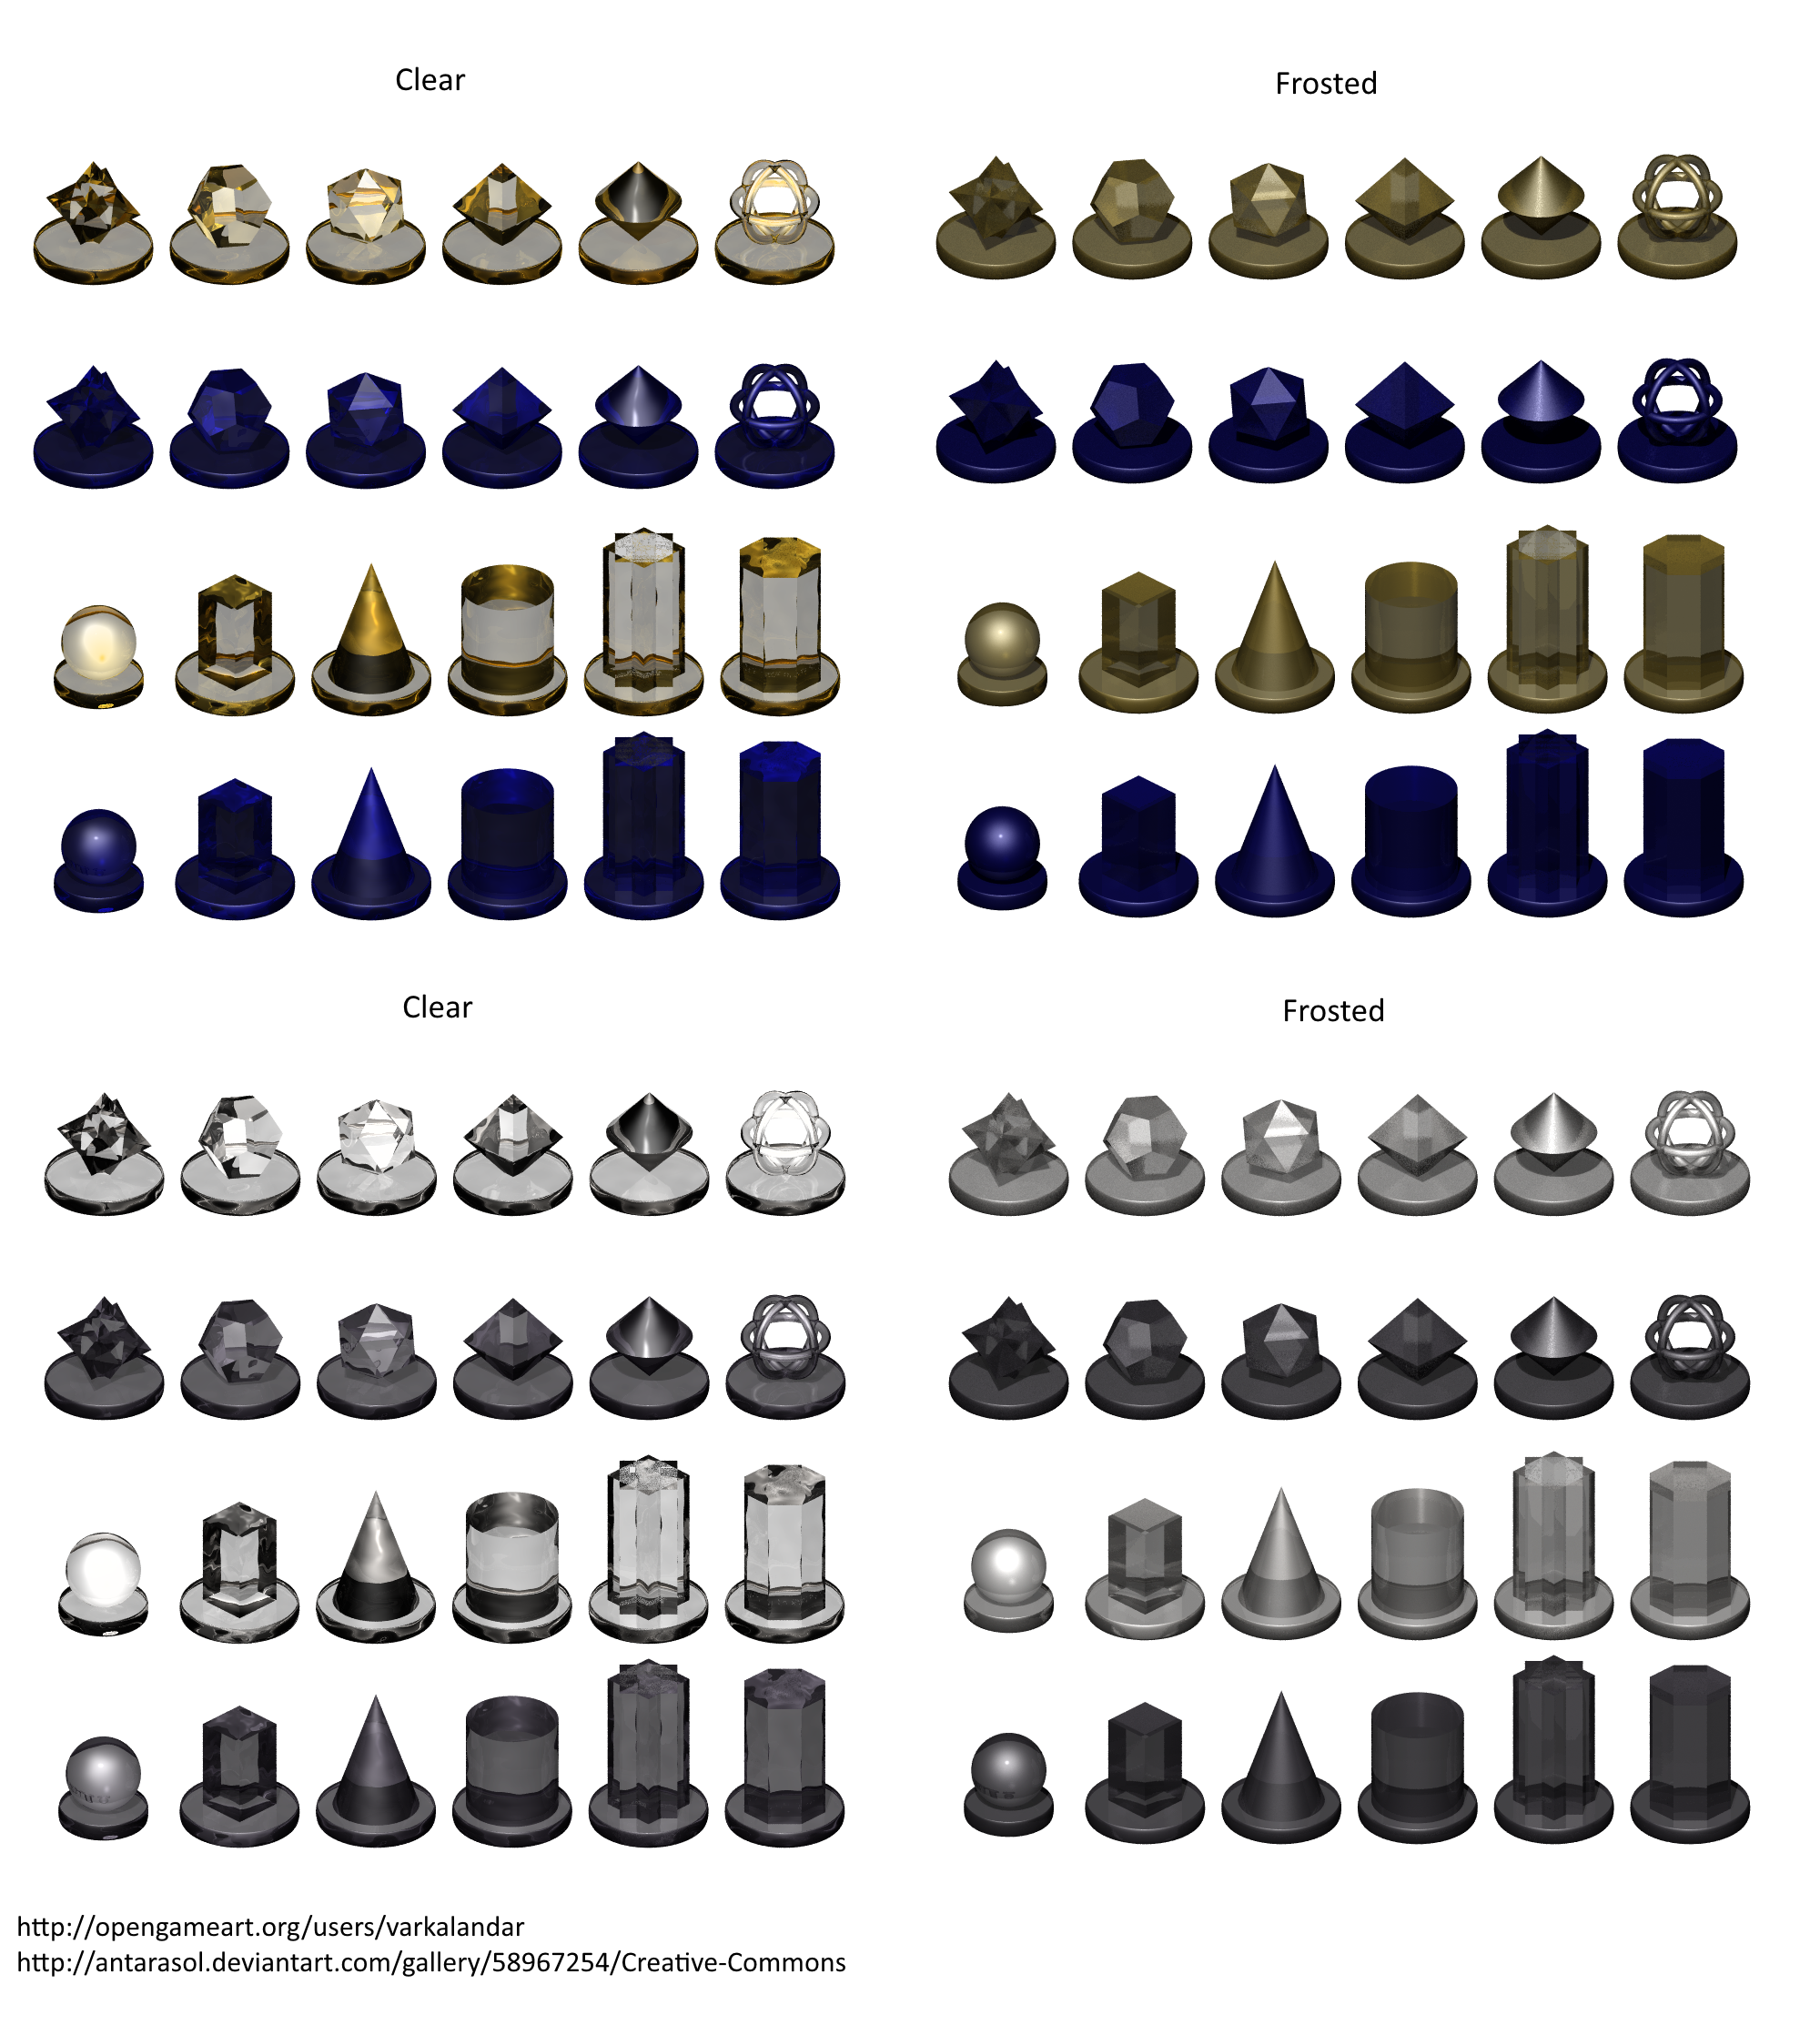
\includegraphics[width=6cm]{Images/pions.png}
        \caption{Textures pour les pions}
        \label{fig:textures_pions}
    \end{figure}
    
    % 
\includegraphics[width=4cm]{Images/soldier.png}
    
    \begin{figure}[!htbp]
        \centering
        
\includegraphics[width=14cm]{Images/cartes.png}
        \caption{Textures pour les cartes}
        \label{fig:textures_cartes}
    \end{figure}